%%
%% 研究報告用スイッチ
%% [techrep]
%%
%% 欧文表記無しのスイッチ(etitle,eabstractは任意)
%% [noauthor]
%%

%\documentclass[submit,techrep]{ipsj}
\documentclass[submit,techrep,noauthor]{ipsj}

\newcommand{\RQOne}{レビューコメントにおいて修正要求と修正確認は分類可能か}
\newcommand{\RQTwo}{レビューコメントにおいて修正完了の有無を分類することは可能か}
\newcommand{\RQThree}{コードレビュー票単位と修正要求単位に基づく進捗状況評価結果は異なるか}

\newcommand{\todo}[1]{\colorbox{yellow}{{\bf TODO}:}{\color{red} {\textbf{[#1]}}}}
\newcommand{\change}[1]{\colorbox{green}{{\bf CHANGE}:}{\color{blue} {\textbf{[#1]}}}}
\newcommand{\new}[1]{\colorbox{cyan}{{\bf NEW}:}{\color{black} {\textbf{[#1]}}}}

\usepackage[dvipdfmx]{graphicx}
\usepackage{latexsym}
\usepackage{url}
\usepackage{otf}

\def\Underline{\setbox0\hbox\bgroup\let\\\endUnderline}
\def\endUnderline{\vphantom{y}\egroup\smash{\underline{\box0}}\\}
\def\|{\verb|}
%

%\setcounter{巻数}{59}%vol59=2018
%\setcounter{号数}{10}
%\setcounter{page}{1}


\begin{document}


\title{修正要求・確認コメントの自動抽出による\\
コードレビューの進捗状況追跡手法に向けて}

%\etitle{How to Prepare Your Paper for IPSJ SIG Technical Report \\ (version 2018/10/29)}

\affiliate{WU}{和歌山大学\\
Wakayama University}

\author{川\UTF{FA11} 晴斗}{Kawasaki Haruto}{WU}[kawasaki.haruto@g.wakayama-u.jp]
\author{伊原 彰紀}{Ihara Akinori}{WU}
\author{上中 瑞稀}{Uenaka mizuki}{WU}

\begin{abstract}
コードレビュー対象のソースコードが改善を要する場合,検証者は実装者に修正を要求する.ソフトウェア開発においてプロジェクト管理者は,コードレビューの進捗を確認しながら次のリリースに導入可能なソースコードを決定する.しかし大規模なプロジェクトでは,膨大なコードレビューが並行で進められ,個々の進捗を確認することは容易ではない.本研究では,レビューコメントから修正要求コメント,および修正要求が解決されたことを示す修正確認コメントをそれぞれ自動抽出し,コードレビューの進捗状況を追跡する手法を提案する.
\end{abstract}


%
%\begin{jkeyword}
%情報処理学会論文誌ジャーナル,\LaTeX,スタイルファイル,べからず集
%\end{jkeyword}
%
%\begin{eabstract}
%This document is a guide to prepare a draft for submitting to IPSJ
%Journal, and the final camera-ready manuscript of a paper to appear in
%IPSJ Journal, using {\LaTeX} and special style files.  Since this
%document itself is produced with the style files, it will help you to
%refer its source file which is distributed with the style files.
%\end{eabstract}
%
%\begin{ekeyword}
%IPSJ Journal, \LaTeX, style files, ``Dos and Dont's'' list
%\end{ekeyword}

\maketitle

%%%%%%%%%%%%%%%%%%%%%%%%%%%%%%%%%%%%%
%1章はじめに
\section{はじめに}
%%%%%%%%%%%%%%%%%%%%%%%%%%%%%%%%%%%%%

ソフトウェア開発におけるコードレビューは,機能追加や不具合修正のために開発者(実装者)が変更したソースコードを,別の開発者(検証者)が欠陥の有無やコードの可読性を確認する重要な工程である\cite{quality1}\cite{quality2}.特に不特定多数の実装者が参加するオープンソースソフトウェア (OSS) 開発には,多様なコーディングスタイルで実装されたソースコードが提出されるため,複数の検証者によってコードレビューが実施される~\cite{review_process}.コードレビューによってソースコードの改善を要する箇所が発見されれば,検証者は実装者に改善を要求する.

リリースまでのマイルストーンを計画するために,ソフトウェア開発プロジェクトはコードレビューを含めたタスクの進捗を計画し,進捗状況を追跡する~\cite{review_time}.GitHubが提供する機能であるMilestoneは,特定の期限までに完了する必要がある不具合 (Issue) 票やコードレビュー (Pull Request) 票の件数を把握することができ,多くの組織がスケジュールを検討するために使用している.各コードレビュー票の中には,ソースコードの改善要求が含まれ,改善要求を明確に提示できる作業タスクであれば,緻密なマイルストーンを計画することが可能である.しかし,コードレビューでは実装者や他の検証者との間で,ソースコードをさらに改善すべきか判断するために議論することが多く,その結果,コードレビューの時間が長期化している~\cite{review_time1}~\cite{review_time2}.

本研究では,コードレビューにおける進捗状況の把握に向けた第一歩として,検証者がコードレビュー票に投稿したコメントの中から,検証者がコードレビューによって更なる修正を依頼するコメント(修正要求コメント),およびソースコードが修正されたことを検証者が確認したことを伝えるコメント(確認コメント)を自動抽出する手法を提案する.また,GitHubのMilestoneのようにコードレビュー票数に基づく進捗管理と,本研究で開発する修正要求数に基づく進捗管理の違いを示す.

\noindent\textbf{RQ1: \RQOne(\ref{sec:RQ1}章)}\\
RQ1では,検証者が記録するコードレビュー票に残したコメントを修正要求と修正要求が解決されたことを示す修正確認にそれぞれ分類できるか否かを目視調査する.具体的には,OSS開発で公開されているコードレビュー票を無作為抽出し,各コードレビュー票に記録されたレビューコメントを目視調査する.

\noindent\textbf{RQ2: \RQTwo(\ref{sec:RQ2}章)}\\
RQ2では,レビューコメントに対して修正要求や修正確認であるか否かを目視によって分類したデータセットを教師データとし,学習済みモデルBERTをファインチューニングすることで,修正要求や修正確認を分類するモデルを構築する.さらに,修正要求文とその要求が解決されたことを確認する修正確認文の紐づけを試みる.

\noindent\textbf{RQ3: \RQThree(\ref{sec:RQ3}章)}\\
RQ3では,本研究で開発した修正要求コメント,および修正確認コメントの抽出によってコードレビューの進捗状況の追跡結果の違いを示す.

以降,本論文では,\ref{sec:progress}章でOSS開発における進捗確認方法と従来研究について述べる.その後,\ref{sec:RQ1}章でRQ1,\ref{sec:RQ2}章でRQ2,\ref{sec:RQ3}章でRQ3のそれぞれの手法と結果について述べる.そして\ref{sec:discussion}章で結果の考察及び妥当性について述べ,\ref{sec:conclusion}章でまとめる.

%%%%%%%%%%%%%%%%%%%%%%%%%%%%%%%%%%%%%
%2章関連研究
\section{関連研究}\label{sec:progress}
%%%%%%%%%%%%%%%%%%%%%%%%%%%%%%%%%%%%%

大規模OSSの開発では,実装者がコードレビュー依頼をGerritやReview Boardをはじめとしたコードレビュー管理システムの票に記録することで,実装者と検証者が円滑なコミュニケーションを行う~\cite{code_review}.これらのシステムに蓄積されたデータを用いて,コードレビューの作業内容や工数を見積もる研究が行われている.

大規模OSSの開発では,日々膨大なコードレビュー票がプロジェクトに提出されるため,開発者は優先して取り組むコードレビュー票に順位をつけざるを得ない.従来研究では,コードレビュー票の優先順位を決定するための研究が多数取り組まれており,ソフトウェア利用者に悪影響を与えるセキュリティ関連のソースコード変更のコードレビューは優先順位が高く設定されることが明らかにされている~\cite{integrator}\cite{review_prioritize_pineapple}.しかし,その他の急を要さない不具合修正やリファクタリングのために変更されたソースコードのコードレビューは優先順位が日々変動する.Kononenkoらは,開発者へのインタビューにおいて,直近のリリースに導入する変更提案の優先順位はリリースまでの期間によって異なることを明らかにしている\cite{release_merge}.

コードレビューの進捗を計画,追跡することは,リリースまでの緻密なマイルストーンを計画するために重要であり,各コードレビューに要する時間を見積もる研究が行われている~\cite{estimate_time1}\cite{estimate_time2}\cite{estimate_time3}\cite{estimate_time4}\cite{estimate_time5}.
Maddilaらは,コードレビュー対象のソースコード行数,変更内容の種類,コードレビューチケット作成日,ソースコード作成者の特徴など28の特徴量に基づきコードレビュー時間を見積もる手法を提案している\cite{estimate_time2}.

コードレビューの優先順位,およびコードレビューにかかる工数の見積もりに関する従来研究では,コードレビューチケットを提出時に計測できる特徴量に基づいていることが多い.検証者による修正要求に基づき優先順位やコードレビューに要する時間を見積もることで,さらに正確なマイルストーンを計画することができると考える.そこで,本研究では修正要求コメント文を自動抽出する手法を開発し,コードレビューの進捗状況の追跡を試みる.

%%%%%%%%%%%%%%%%%%%%%%%%%%%%%%%%%%%%%
%3章 RQ1:レビューコメントの目視調査
\section{RQ1:\RQOne}\label{sec:RQ1}
%%%%%%%%%%%%%%%%%%%%%%%%%%%%%%%%%%%%%

\subsection{概要}
コードレビュー票には多数のコメントが記録されている.実装者が投稿するコメントには,作成したソースコードの補足,検証者からの質問に対する回答などがある.検証者が投稿するコメントには,実装者への修正要求,提出されたパッチへの問い,修正要求が解決したことの確認などがある.RQ1では,コードレビュー票に記録されたコメントの中から,検証者がコードレビューによって更なる修正を依頼するコメント(修正要求コメント)か否か,ソースコードが修正されたことを検証者が確認したことを伝えるコメント(確認コメント)か否か,をそれぞれ分類できるか否かを目視調査する.

\subsection{データセット}
RQ1では,OpenStackのコアコンポーネントであるNova,Neutron,Cinder,Keystone,Swift,Glanceの6つのプロジェクト,およびOpenStackにおける大規模プロジェクトであるHorizonの合計7つのプロジェクトを分析対象とする.OpenStackプロジェクトでは,レビュー管理システムとしてGerritを使用しており,各コードレビュー票に開発者からのコメント投稿数が多いため,多くの従来研究がコードレビュー過程を分析する調査対象としている.本研究では,分析対象とするプロジェクトの立ち上げ時から2022年9月までにリポジトリに導入されたコードレビュー票に記録されるコメントを収集する.表\ref{table:NumberOfProjects}は,各プロジェクトのコードレビュー票数,コメント数を示す.プロジェクト毎のコードレビュー票の平均コメント数は22件から87件である.

%-----------------------
\begin{table}[t]
\centering
  \caption{各プロジェクトにおいて導入されたコードレビュー票数とコメント数}
  \vspace{+1mm}
  \label{table:NumberOfProjects}
  \scalebox{1.0}{   
  \begin{tabular}{l|r|r}  \hline \hline
    \multicolumn{1}{c|}{プロジェクト} & \multicolumn{1}{c|}{コードレビュー票数} & \multicolumn{1}{c}{コメント数}\\ \hline
    Nova & 29,338 & 1,571,114\\ 
    Neutron & 18,665 & 1,106,829\\ 
    Cinder & 12,917 & 1,127,176\\ 
    Horizon & 9,645 & 209,681\\ 
    Keystone & 8,270 & 190,464\\ 
    Swift & 6,172 & 112,709\\ 
    Glance & 4,545 & 102,360\\ \hline
    合計 & 89,552 & 4,420,333\\ \hline
  \end{tabular}
  }
\end{table}
%-----------------------

%-----------------------
\begin{table*}[t]
\centering
  \caption{修正要求に含まれていた内容}
  \label{table:request_sum}
  \scalebox{1.1}{   
  \begin{tabular}{l|l|r}  \hline \hline
    \multicolumn{1}{c|}{修正要求内容} & \multicolumn{1}{c|}{コメント例} & \multicolumn{1}{c}{件数(重複可)}\\ \hline
    機能改善 & better to use mock instead of stub & 345\\ \hline
    リファクタリング/コード整形 & Could you use rstrip instead? & 278\\ \hline
    コード外の修正(コミットメッセージ等) & commit message line should have less than 72 characters & 233\\ \hline
    バグ修正 & need to address failures in unit tests & 92\\ \hline
    誤字修正 & fileds -\textgreater fields & 47\\ \hline
  \end{tabular}
  }

\vspace{2mm}

\centering
  \caption{修正確認に含まれていた内容}
  \label{table:achieve_sum}
  \scalebox{1.15}{   
  \begin{tabular}{l|l|r}  \hline \hline
    \multicolumn{1}{c|}{修正確認内容} & \multicolumn{1}{|c}{コメント} & \multicolumn{1}{|c}{件数(重複無)} \\ \hline
    強い承認 & Looks good to me, approved または Code-Review+2 & 666 \\ \hline
    弱い承認 & Looks good to me, but someone else must approve または Code-Review+1 & 893 \\ \hline
    その他 & Good Change や Thank you や Nice など & 315 \\
    % & I would prefer this is not submitted as is または \\ Code-Review-1 & 弱い非承認 \\ \hline
    % This shall not be submitted または \\ Code-Review-2& 強い非承認 \\ 
    \hline
  \end{tabular}
  }
\end{table*}
%-----------------------

\subsection{手法}
分析対象とする7プロジェクトを区別せずに89,552件のコードレビュー票から信頼区間95\%,許容誤差5\%となる383件を無作為に選択し,コードレビュー票に投稿されたコメント12,086件を目視調査する.具体的には,修正要求のコメント,および修正確認のコメントを抽出する.ただし,ボットによるテスト実行結果は修正要求,修正確認と判定しない.

\subsection{結果}

表~\ref{table:request_sum}および表\ref{table:achieve_sum}は,分析対象とする12,086件のコメントから修正要求コメントか否か,修正確認コメントか否か,を内容に基づき目視分類した結果を示す.

表~\ref{table:request_sum}の結果から,12,086件のレビューコメントのうち,874件(約7.2\%)が修正要求コメントであった.それぞれの修正要求コメントは5パターン(機能改善,リファクタリング,コード外の修正,バグ修正,誤字修正)に分類でき,検証者によって記述されることが多いパターンは機能改善,リファクタリング,コード外の修正であることを確認した.その他には,変更されたソースコードに欠陥が含まれるバグ修正や誤字修正の依頼が含まれていた.検証者によって記述された修正要求コメントには,表~\ref{table:request_sum}に示す他にも\textit{``Need a space before 5.''}や\textit{``This could use a bit more explanation in the commit message.''},\textit{``Please fix the pep8 errors''}のように\textit{``need''},\textit{``could''},\textit{``please''}などの自然言語で一般的に要求を表す単語が多く用いられていた.
Gerritでは,検証者がコードレビューのコメントに評価結果を表すラベルの付与を示す機能を有している.具体的には,変更内容に賛成していることを表すラベルとして\textit{``Looks good to me, approved(Code-Review+2)''}や\textit{``Looks good to me, but someone else must approve(Code-Review+1)''}などがある.また,変更内容に反対していることを表すラベルとして\textit{``I would prefer that you didn't submit this''}や\textit{``I would prefer that you didn't merge this''}などがある.ただし,たとえ変更内容に賛成していても修正要求を併記していることもある.本分析では変更内容に賛成していても修正要求が併記されているコメントを92件(約6%)を確認したため,検証評価ラベルのみで要求ありを分類することはできない.

次に表\ref{table:achieve_sum}の結果から,12,086件のレビューコメントのうち,1,874件(約15.5\%)が修正確認コメントであった.1,874件の修正確認コメントのうち,83.2\%はOpenStackで提供されている変更提案に対する承認を表すラベルがレビューコメントに付与されていることを確認した.また,検証評価ラベル以外の修正確認コメントとして,\textit{``Good Change''}や\textit{``Thank you''}などの感謝を示すコメントを投稿する検証者も複数確認した.

%著者が修正確認として判断したコメントのうち,83.2\%はOpenStackで提供されている変更提案に対する承認を表す検証評価ラベルがレビューコメントに付与されていることを確認した.検証評価ラベルはGerritで提供される機能の一つで,コードレビュー結果をスコアで評価を提示することができる.表\ref{table:achieve_sum}に示す強い承認または,弱い承認を表すコメントは検証評価ラベルである.また,Gerritの機能ではなく,検証者がコメントとして``Good Change''や``Thank you''などを投稿していることも確認した.

%また,修正要求が修正確認と紐づいているかの実情を確認した結果,修正要求を提出した検証者が後に修正確認をしていないこともあり,修正要求と修正確認が一対一対応していないことも存在していた.

これらの結果からレビューコメントにおける修正要求または修正確認には特徴があることを確認したため,修正要求や修正確認は機械的な手法でレビューコメントから抽出できることが示唆される.

%%%%%%%%%%%%%%%%%%%%%%%%%%%%%%%%%%%%%
%4章 RQ2:修正要求/確認の抽出と紐付け
\section{RQ2:\RQTwo}\label{sec:RQ2}
%%%%%%%%%%%%%%%%%%%%%%%%%%%%%%%%%%%%%

\subsection{概要}
RQ2では,RQ1で目視で抽出した修正要求コメント874件と修正確認コメント1,874件のデータセットを用いて,学習済みモデルBERTをファインチューニングし,レビューコメントに修正要求,および修正確認を含むか否かを機械的に特定するモデルを構築し,評価する.

\subsection{手法}

%-------------------
\begin{figure*}[t]
\centerline{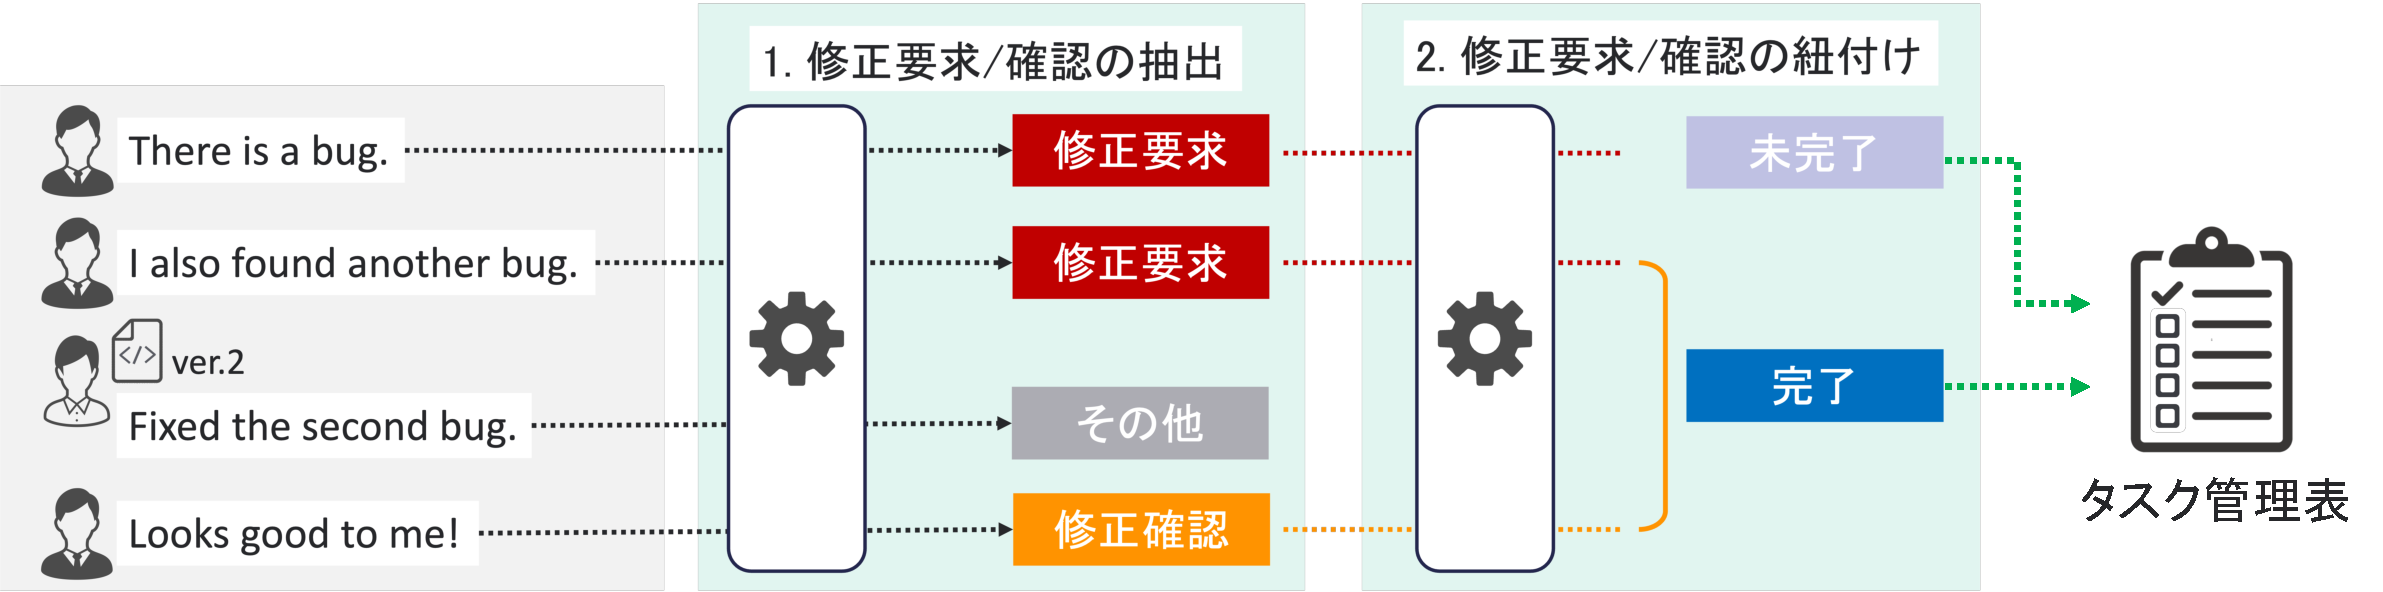
\includegraphics[width=1.0\linewidth]{Kawasaki_fig/research_method.pdf}}
\caption{コードレビューの進捗状況追跡手法}
\label{fig:research_method}
\end{figure*}
%-------------------

\subsubsection{修正要求の抽出}
本研究の手法を図\ref{fig:research_method}に示す.コードレビューの進捗状況追跡のため,レビューコメントから修正要求及び修正確認を抽出する.まず,レビューコメントから修正要求を抽出するため,\ref{sec:RQ1}章で目視調査したデータセットを教師データとして用い,自然言語モデルBERT\footnote{BERT: \url{https://huggingface.co/docs/transformers/ja/model_doc/bert}}をファインチューニングしたモデルでレビューコメントに修正要求を含むか否かを判定する.目視調査した12,086件を5分割し,1つをテスト用のデータに用いて,残りの4つを訓練用のデータに用いる5分割交差検証を行う.訓練用のデータは,さらに7:3の割合で分割して学習用と検証用に用いる.モデル作成時のパラメータは学習時のパッチサイズが8,評価時のパッチサイズが16,エポック数が3,ウォームアップステップ数が500,重み減衰が0.01とした.評価指標には適合率,再現率,F1値を用い,交差検証で5回実行した結果の中央値でモデルの有用性を評価する.また,Gerriが提供する検証評価ラベルが分類に与える影響を確認するため,同様の設定のモデルをラベルを含むコメントからラベルを削除したコメントだけをテストデータに用いて評価を行う.

\subsubsection{修正確認の抽出}
図\ref{fig:research_method}に示すようにレビューコメントから修正確認を抽出する.修正確認は修正要求と異なり言語的表現が少なく,Gerritで提供されているコードレビューの結果を示すラベルや``LGTM''のように定型的な表現がなされていることが多い.そこで表\ref{table:achieve_sum}の「その他」に分類した語彙を含むコメントを抽出したところ,\textit{``LGTM''},\textit{``Looks good''},\textit{``Looks ok''}を含むコメントのみレビューコメントを修正確認と分類した割合が90\%を超えていることを確認した.そこで本研究での修正確認として用いるコメント群は表\ref{table:achieve_sum}で示す強い承認,弱い承認つまり,Gerritで提供されているコードレビュー結果のスコア及び\textit{``LGTM''},\textit{``Looks good''},\textit{``Looks ok''}を含むコメントとする.

\subsubsection{修正要求と修正確認の紐付け}
修正要求に基づき修正されたソースコードが確認されたとき,検証者は修正確認コメントを投稿することがある.しかし,RQ1で目視によって修正要求に対する修正確認が投稿されているか否かを確認したところ,必ずしも修正要求コメントを投稿した検証者が,修正確認コメントを投稿しているとは限らないことがわかった.また,複数人の異なる検証者が修正要求コメントを投稿し,ソースコードが修正された後に,いずれか一人の検証者が全ての要求に対する修正が完了していることを確認していることもある.
そこで本研究では進捗状況評価を行うための第一歩として,図\ref{fig:research_method}に示す修正要求と修正確認の紐付けには修正要求と後のパッチで提出された修正確認を2つの定義で行う.
\begin{itemize}
\item 修正確認コメントを投稿した検証者が,以前に投稿した要求は全て検証されたものとみなす
\item 修正確認コメントを投稿以前の要求は全て検証されたものとみなす
\end{itemize}

%そこで本研究では進捗状況評価を行うための第一歩として,修正要求コメントの投稿後に提出された修正確認コメント(``LGTM'',``Looks good'',``Looks ok'')に全て紐づける.

\subsection{結果}
\subsubsection{修正要求コメントの予測結果}
表\ref{table:label_score}は,本研究でBERTをファインチューニングした予測モデルによって修正要求コメントを予測した結果を示す.5分割交差検証の結果,適合率が0.84,再現率0.78,F値0.81となった.この結果から修正要求コメントを高い精度で予測できることを明らかにした.現時点で,予測モデルの結果の比較対象となる手法を検討できていないため十分な有用性の評価を示すことができていないが,今後の研究では,自然言語として要求文を特定する既存手法との比較を検討する.

また,表\ref{table:label_score}には,Gerritが提供する検証評価ラベルを含むコメントからラベルを削除したコメントだけをテストデータに用いた評価結果も示す.Code-Review-1は修正要求を含むコメントが多量に存在するため,全ての評価指標で高いことがわかる.しかし,Code-Review+1やCode-Review+2では一般的に修正内容に賛同しているが,要求を併記していることもあるために再現率が低下したと示唆される.

%-----------------------
\begin{table}[t]
\centering
  \caption{修正要求コメントの予測精度}
  \label{table:label_score}
  \scalebox{1.00}{   
  \begin{tabular}{l|r|r|r}  \hline \hline
    \multicolumn{1}{c|}{スコア(件数)} & \multicolumn{1}{c|}{適合率} & \multicolumn{1}{c|}{再現率} & \multicolumn{1}{c}{F値}\\ \hline
    全レビューコメント(12,086件) & 0.84 & 0.78 & 0.81\\ \hline    
    Code-Review-2(14件) & 0.20 & 1.00 & 0.33\\ 
    Code-Review-1(465件) & 0.97 & 0.97 & 0.96\\ 
    Code-Review+1(918件) & 0.78 & 0.70 & 0.69\\ 
    Code-Review+2(916件) & 0.60 & 0.64 & 0.63\\ \hline
  \end{tabular}
  }
\end{table}
%-----------------------

次に,表\ref{table:request_accuracy}は,RQ1にて分類した修正要求内容別の再現率を示す.修正要求内容が200件以上存在する機能改善,リファクタリング/コード整形は,再現率が8割以上であることを確認した.
%それ以外の修正要求も7割以上ではあったが,コード外の修正依頼には表現にばらつきがあるため,再現率が落ちてしまったと示唆する.
また,コード外の修正やバグ修正,誤字修正の修正要求の再現率はすべて7割以上であるものの,機能改善やリファクタリング/コード整形と比べると再現率が低下した.この理由として,コード外の修正はコミットメッセージの修正や変更に対するパッチの分割要求など,修正要求の対象が多岐にわたっていることが起因していると示唆する.
%誤字修正は,RQ1の目視分析を通して他の修正要求より定型的な表現を用いられていることが多かったが,再現率が8割未満であり,データセットの中に誤字修正に関する要求が少ないことが起因していると示唆する.
また,バグ修正や誤字修正は,RQ1の目視分析を通して他の修正要求より定型的な表現を用いられていることが多かったが,データセットの中にバグ修正や誤字修正に関する要求が少ないことが再現率の低下に起因していると示唆する.

%-----------------------
\begin{table}[t]
\centering
  \caption{修正要求内容毎の再現率}
  \label{table:request_accuracy}
  \scalebox{1.1}{
  \begin{tabular}{l|r}  \hline \hline
    \multicolumn{1}{c|}{修正要求内容} & \multicolumn{1}{c}{再現率(\%)}\\ \hline
    機能改善 & 80.7\\ 
    リファクタリング/コード整形 & 85.3\\ 
    コード外の修正(コミットメッセージ等) & 75.5\\ 
    バグ修正 & 73.9\\ 
    誤字修正 & 78.7\\ \hline
  \end{tabular}
  }
\end{table}
%-----------------------

\subsubsection{修正確認コメントの予測結果}

%-----------------------
\begin{table}[t]
\centering
  \caption{修正確認コメントの予測精度}
  \label{table:confirm_score}
  \scalebox{1.00}{   
  \begin{tabular}{l|r|r|r}  \hline \hline
    \multicolumn{1}{c|}{スコア(件数)} & \multicolumn{1}{c|}{適合率} & \multicolumn{1}{c|}{再現率} & \multicolumn{1}{c}{F値}\\ \hline
    全レビューコメント(12,086件) & 0.94 & 0.97 & 0.96\\ \hline    
  \end{tabular}
  }
\end{table}
%-----------------------

表\ref{table:confirm_score}は,本研究で修正確認コメントを特定するとして用いる基準による結果を示す.評価実験の結果,再現率が97.3\%であった.\textit{``LGTM''}以外にも\textit{``Thank you''}による修正確認もあるが,修正確認以外にも使われる用語のため,再現率が100\%に至っていない.

%次に,承認を表すラベルか信頼度が90\%を超えコメントのいずれかが含まれているコメントを修正確認として扱ったところ,レビューコメントのうち修正確認として分類されたコメントの97.3\%を修正確認として分類可能なことを確認した.

\subsubsection{修正要求と修正確認の紐付け}

%RQ1で目視調査したレビューコメント12,086件を訓練用,検証用に7:3の割合で分割してモデルを構築し,
表\ref{table:link_ratio}は,89,552件の変更提案から239,286件の修正要求を抽出し,4.2.3項で定義した方法で修正要求と修正確認とを紐付けた結果を示す.修正要求提出者が後のパッチで修正確認を行うことは4割程度であり,多くの検証者が修正要求に対して改修後,修正確認コメントを投稿していないことが示唆される.ただし,検証者を問わなければ約8割で修正確認が行われていることが示唆される.

%最後に,修正要求の抽出用に作成したモデルを用いた.目視調査した12,086件のレビューコメントを訓練用,検証用に7:3の割合で分割してモデルを構築し,89,552件の変更提案から239,286件の修正要求を抽出した.また,定義した修正要求が提出されたパッチより後に存在する修正確認と紐付けを行ったところ207,111件が紐づくことを確認した.

%-----------------------
\begin{table}[t]
\centering
  \caption{定義毎に修正要求(239,286件)と紐づいた割合}
  \label{table:link_ratio}
  \scalebox{1.2}{   
  \begin{tabular}{l|r|r}  \hline \hline
    \multicolumn{1}{c|}{紐付けの定義} & \multicolumn{1}{c|}{件数} & \multicolumn{1}{c}{割合(\%)}\\ \hline
    修正要求提出者が修正確認 & 110,042 & 45.8\\ 
    検証者を問わず修正確認 & 207,997 & 86.6\\ \hline
  \end{tabular}
  }
\end{table}
%-----------------------

%%%%%%%%%%%%%%%%%%%%%%%%%%%%%%%%%%%%%
%5章 RQ3:従来の進捗状況評価との比較
\section{RQ3:\RQThree}\label{sec:RQ3}
%%%%%%%%%%%%%%%%%%%%%%%%%%%%%%%%%%%%%

\subsection{概要}
RQ2ではデータセットに対して修正要求と修正確認を抽出し,それぞれを対応したコメント同士で紐付けを行なった.RQ3では従来研究と同様にコードレビュー票の件数に基づき完了していないコードレビューの進捗状況を分析した結果と,修正要求の件数に基づいてコードレビューの進捗状況を分析した結果を比較する.

%ただし,紐付けの定義としてはRQ2での「検証者を問わず後のパッチで修正確認」を用いることとする.

\subsection{分析手法}
RQ2で抽出した修正要求コメント239,286件に対して,1日毎に完了していない(GerritのStatusがMergedやAbandonedでない)コードレビュー票の件数とRQ2で定義した修正確認コメント「修正確認コメントを投稿以前の要求は全て検証されたものとみなす」に基づき,修正確認されていない修正要求の件数の分布を分析する.ただし,修正確認と紐づかなかった修正要求はその修正要求を含む変更提案が導入された時点で修正要求は満たされたこととする.

%3.3章のデータセットを用いて,1日毎に存在したコードレビュー票の件数と修正要求の件数の分布に有意差が存在するかを検証する.

\subsection{結果}
図\ref{fig:task_dist}は,1日毎に存在したコードレビュー票の件数と修正要求の件数の分布を示す.NeutronやCinder,Keystoneは他のプロジェクトと比較しても特に中央値や外れ値の分布がコードレビュー票と修正要求で分布が異なっている.表\ref{table:Mann-White}はプロジェクト毎の1日あたりの変更提案数と修正要求数を有意水準は5\%としてMann-WhitneyのU検定の結果を示す.全てのプロジェクトの分布で統計的に有意な差があり,1つのコードレビューにおいて修正要求コメントが複数存在していることが多い.したがって,コードレビュー票の件数のみでリリーススケジュールを立案すると,期待よりも修正要求数が多いコードレビュー票において誤差が生じることが示唆される.

図~\ref{fig:task_trans}は,一例としてKeystoneプロジェクトを対象に,検証が完了していないコードレビュー票数の推移と,修正確認されていない修正要求数の推移を示す.図~\ref{fig:task_trans}から,2011年から2014年,2018年から2020年では,検証が完了していないコードレビュー票数と修正確認されていない修正要求数がほぼ同じであるため,コードレビュー票1件に修正要求が1件程度であることが示唆される.一方で,それ以外の2015年から2017年ではコードレビュー票1件に対して修正要求が2件以上であることが示唆される.この時期は,修正要求数が多い時期であったことがわかる.ただし,本研究では修正要求の修正にかかる時間的コストや修正の難しさを考慮できていない.今後は,修正要求の修正にかかるコストを考慮することで,リリーススケジュールへの影響を明らかにできると考える.

%p値の結果から全てのプロジェクトで分布には有意差があり,コードレビュー票の件数と修正要求の件数の分布が異なることを確認した.また,効果量を比較すると,Keystoneが0.473という最も高い値を算出した.そこでKeystoneのコードレビュー票の開放数の推移と修正要求の開放数の推移を図~\ref{fig:task_trans}に示す.
%修正要求はコードレビュー票と比べて開放数の変動が大きく,コードレビュー票を確認するだけでは追跡できなかった進捗状況を追跡可能であることが示唆される.

%-----------------------
\begin{table}[t]
\centering
  \caption{プロジェクト毎の1日あたりの変更提案数と修正要求数の分布}
  \label{table:Mann-White}
  \scalebox{1.2}{   
  \begin{tabular}{l|r}  \hline \hline
    \multicolumn{1}{c|}{プロジェクト} & \multicolumn{1}{c}{p値}\\ \hline
    Neutron & 1.14e-40\\ 
    Nova & 5.60e-39\\ 
    Glance & 5.14e-07\\ 
    Cinder & 2.81e-18\\ 
    Swift & 2.78e-64\\ 
    Horizon & 5.87e-07\\ 
    Keystone & 1.15e-05\\ \hline
  \end{tabular}
  }
\end{table}
%-----------------------

%-------------------
\begin{figure}[t]
\centerline{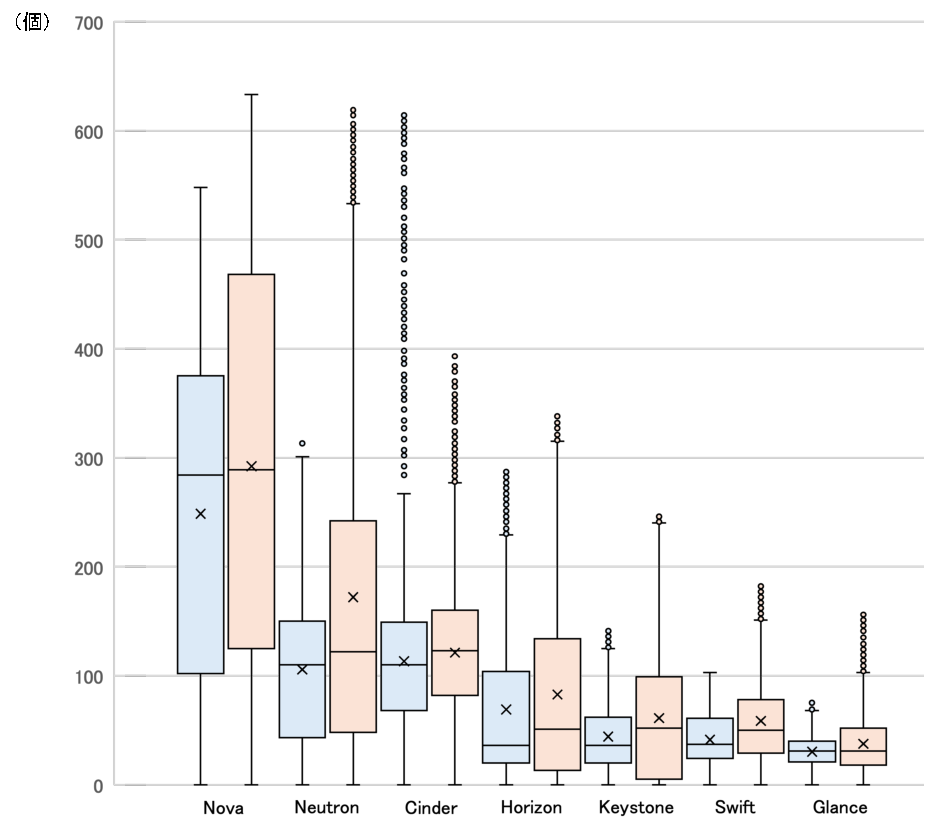
\includegraphics[width=1.0\linewidth]{Kawasaki_fig/task_dist.pdf}}
\caption{1日毎の存在するコードレビュー票の件数と修正要求の件数の分布(左:コードレビュー票, 右:修正要求)}
\label{fig:task_dist}

\vspace{2mm}

\centerline{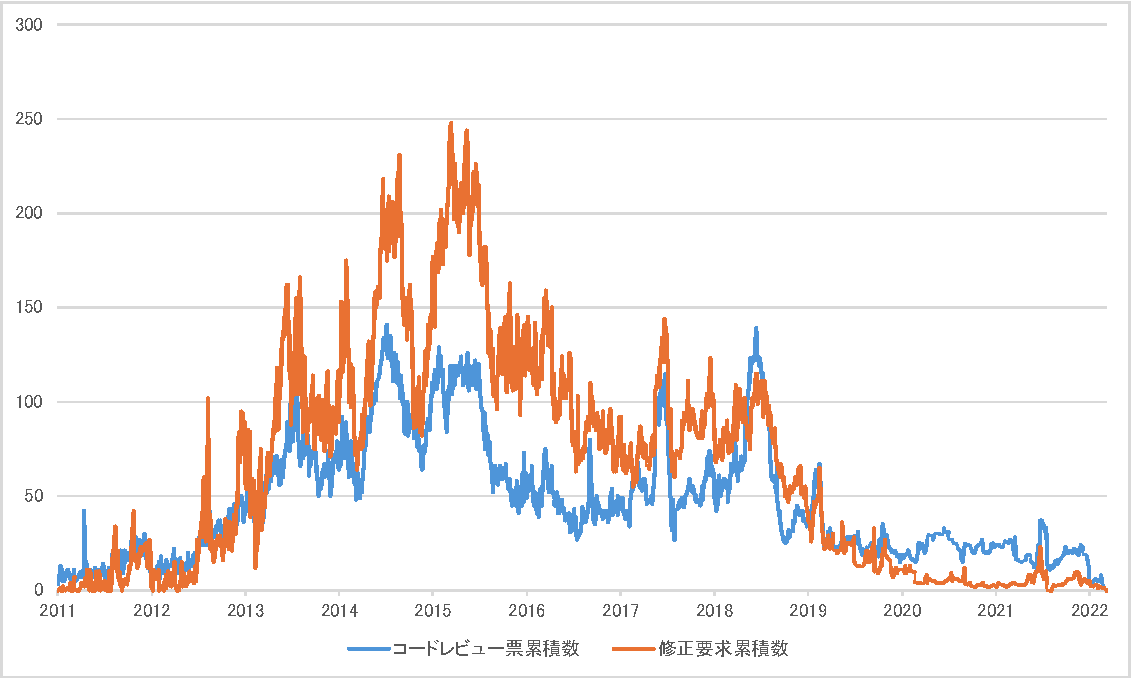
\includegraphics[width=1.0\linewidth]{Kawasaki_fig/task_trans.pdf}}
\caption{Keystoneのコードレビュー票と修正要求の開放数の推移}
\label{fig:task_trans}
\end{figure}
%-------------------

%%%%%%%%%%%%%%%%%%%%%%%%%%%%%%%%%%%%%
%6章
\section{妥当性の脅威}\label{sec:discussion}
%%%%%%%%%%%%%%%%%%%%%%%%%%%%%%%%%%%%%
\subsection{内的妥当性}
本研究ではレビューコメント修正要求か否か,修正確認か否かを著者が目視によって判断している.目視による分類結果は,他者の評価基準によって分類が異なる可能性がある.今後は複数人による目視分類を実施することで,分類の信頼度の向上させる.
%修正要求は修正を求める内容であることを明確に伝えられなければ実装者に修正されない可能性が発生するため,修正要求と分類した多くのコメントは他者の分類結果と一致することが示唆される.同様に修正確認も明確に伝える内容でなければ,プロジェクトへの導入に時間を要する可能性が発生するため,多くの修正確認と分類したコメントは他者の分類結果っと一致することが示唆される.

また,修正確認の定義としてGerritで提供されているコードレビュー結果のスコア及び\textit{``LGTM''},\textit{``Looks good''},\textit{``Looks ok''}を含むコメント群を用いたが,実際には\textit{``Good Change''}や\textit{``Thank you''}のような他の表現を用いた修正確認が存在する.しかし,定義した修正確認コメント群は著者が分類した修正確認のうちF値が0.96と高い値であることから他の表現による修正確認による影響は小さいと示唆される.

また,紐付けの定義として二つの定義を提示したが,実際には定義に基づかない紐付き方も存在する.しかし,修正確認コメントが高い割合で抽出可能なことから紐付き方による影響は小さいと示唆する.

\subsection{外的妥当性}
本研究では,OpenStackのコアコンポーネントの6つのプロジェクトと大規模プロジェクトであるHorizonを対象とした.対象として用いるプロジェクトや期間によっては予測精度や分析結果が異なることが示唆される.しかし,OpenStackプロジェクトでは,各コードレビュー票に開発者からのコメント投稿数が多いため,データセットとするプロジェクトや期間の変更による予測精度や分析結果への影響は小さいと示唆する.

%%%%%%%%%%%%%%%%%%%%%%%%%%%%%%%%%%%%%
\section{おわりに}\label{sec:conclusion}
%%%%%%%%%%%%%%%%%%%%%%%%%%%%%%%%%%%%%

本研究では,コードレビュー票に記録される修正要求コメント,および修正確認コメントに基づく進捗状況を把握する手法を提案し,3つのRQを検証した.その結果,BERTを用いた手法で修正要求を高い精度で抽出可能であることを確認した.また,1件のコードレビューにおいて,複数の修正要求を含んでいることが多く,コードレビュー票の件数のみでリリーススケジュールを立案すると,期待よりも修正要求数が多いコードレビュー票において誤差が生じることが示唆される.

今後は,修正要求コメントの詳細な分析を行い,多様な修正要求コメントを抽出可能なモデル構築を目指す.
%BERTの予測精度向上に向けてレビューコメントの前処理の手法を確立する.具体的には修正要求と修正要求でない内容が含まれるレビューコメントにおいて修正要求でない内容によって修正要求の予測精度が低下していると考えられるコメントが存在するため,レビューコメントを細分化する手法の確立を目指す.
また,進捗状況を追跡するためには修正にかかる時間的コストや修正の難しさを考慮する必要があるため,修正要求を種類毎に分類する手法の確立も目指す.

%================
%\section*{参考文献}
%================
\bibliographystyle{junsrt}
\bibliography{KawasakiFOSE}

\end{document}